
%%%%%%%%%%%%%%%%%%%%%%%%%%%%%%%%%%%%%%%%%%%%%%%%%%%%%%%%%%%%%%%%%%%%%%%%%%%%%%%%%%%%%%%
%%%%%%%%%%%%%%%%%%%%%%%%%%%%%%%%%%%%%%%%%%%%%%%%%%%%%%%%%%%%%%%%%%%%%%%%%%%%%%%%%%%%%%%
% 
% This top part of the document is called the 'preamble'.  Modify it with caution!
%
% The real document starts below where it says 'The main document starts here'.

\documentclass[12pt]{article}

\usepackage{amssymb,amsmath,amsthm}
\usepackage[top=1in, bottom=1in, left=1.25in, right=1.25in]{geometry}
\usepackage{fancyhdr}
\usepackage{enumerate}
\usepackage{listings}
\usepackage{graphicx}
\usepackage{float}
% Comment the following line to use TeX's default font of Computer Modern.
\usepackage{times,txfonts}



\makeatletter
\renewcommand*\env@matrix[1][*\c@MaxMatrixCols c]{%
  \hskip -\arraycolsep
  \let\@ifnextchar\new@ifnextchar
  \array{#1}}
\makeatother

\newtheoremstyle{homework}% name of the style to be used
  {18pt}% measure of space to leave above the theorem. E.g.: 3pt
  {12pt}% measure of space to leave below the theorem. E.g.: 3pt
  {}% name of font to use in the body of the theorem
  {}% measure of space to indent
  {\bfseries}% name of head font
  {:}% punctuation between head and body
  {2ex}% space after theorem head; " " = normal interword space
  {}% Manually specify head
\theoremstyle{homework} 

% Set up an Exercise environment and a Solution label.
\newtheorem*{exercisecore}{Exercise \@currentlabel}
\newenvironment{exercise}[1]
{\def\@currentlabel{#1}\exercisecore}
{\endexercisecore}

\newcommand{\localhead}[1]{\par\smallskip\noindent\textbf{#1}\nobreak\\}%
\newcommand\solution{\localhead{Solution:}}

%%%%%%%%%%%%%%%%%%%%%%%%%%%%%%%%%%%%%%%%%%%%%%%%%%%%%%%%%%%%%%%%%%%%%%%%
%
% Stuff for getting the name/document date/title across the header
\makeatletter
\RequirePackage{fancyhdr}
\pagestyle{fancy}
\fancyfoot[C]{\ifnum \value{page} > 1\relax\thepage\fi}
\fancyhead[L]{\ifx\@doclabel\@empty\else\@doclabel\fi}
\fancyhead[C]{\ifx\@docdate\@empty\else\@docdate\fi}
\fancyhead[R]{\ifx\@docauthor\@empty\else\@docauthor\fi}
\headheight 15pt

\def\doclabel#1{\gdef\@doclabel{#1}}
\doclabel{Use {\tt\textbackslash doclabel\{MY LABEL\}}.}
\def\docdate#1{\gdef\@docdate{#1}}
\docdate{Use {\tt\textbackslash docdate\{MY DATE\}}.}
\def\docauthor#1{\gdef\@docauthor{#1}}
\docauthor{Use {\tt\textbackslash docauthor\{MY NAME\}}.}
\makeatother

% Shortcuts for blackboard bold number sets (reals, integers, etc.)
\newcommand{\Reals}{\ensuremath{\mathbb R}}
\newcommand{\Nats}{\ensuremath{\mathbb N}}
\newcommand{\Ints}{\ensuremath{\mathbb Z}}
\newcommand{\Rats}{\ensuremath{\mathbb Q}}
\newcommand{\Cplx}{\ensuremath{\mathbb C}}
%% Some equivalents that some people may prefer.
\let\RR\Reals
\let\NN\Nats
\let\II\Ints
\let\CC\Cplx

%%%%%%%%%%%%%%%%%%%%%%%%%%%%%%%%%%%%%%%%%%%%%%%%%%%%%%%%%%%%%%%%%%%%%%%%%%%%%%%%%%%%%%%
%%%%%%%%%%%%%%%%%%%%%%%%%%%%%%%%%%%%%%%%%%%%%%%%%%%%%%%%%%%%%%%%%%%%%%%%%%%%%%%%%%%%%%%
% 
% The main document start here.

% The following commands set up the material that appears in the header.
\doclabel{Math 410: Homework 1}
\docauthor{Stefano Fochesatto}
\docdate{\today}

\begin{document}



\section*{Exercises 1.1}

\begin{exercise}{5(b)} Write the following in the form of $a + bi$
    \begin{equation*}
        (8 + i)-(5 + i)
    \end{equation*}
    \solution By the addition and subtraction of complex numbers we get, 
    \begin{equation*}
        (8 + i)-(5 + i) = (8 - 5) + (1 - 1)i = 3 + 0i
    \end{equation*}
\end{exercise}
\vspace{1in}


\begin{exercise}{6(a)} Write the following in the form of $a + bi$
    \begin{equation*}
        (-1 + i)^2
    \end{equation*}
    \solution By the multiplication of complex numbers we get, 
    \begin{equation*}
        (-1 + i)^2 =  (-1 + i)(-1 + i) = ((-1)(-1)-(1)(1)) + ((-1)(1) + (-1)(1))i = 0 - 2i
    \end{equation*}
\end{exercise}
\vspace{1in}



\begin{exercise}{7(b)} Write the following in the form of $a + bi$
    \begin{equation*}
        \dfrac{-1 + 5i}{2 + 3i}
    \end{equation*}
    \solution By the division of complex numbers we get, 
    \begin{equation*}
        \dfrac{-1 + 5i}{2 + 3i} = \dfrac{(-1)(2) + (5)(3)}{2^2 + 3^2} +  \dfrac{(5)(2) - (-1)(3)}{2^2 + 3^2}i = 1+1i
    \end{equation*}
\end{exercise}
\vspace{1in}

\begin{exercise}{12} Write the following in the form of $a + bi$
    \begin{equation*}
        (2+i)(-1-i)(3+2i)
    \end{equation*}
    \solution By the associative law of multiplication and the multiplication of complex numbers we get the following, 
    \begin{align*}
        (2+i)(-1-i)(3+2i) &= ((2+i)(-1-i))3+2i),\\
        &= (-1 + -3i)(3+2i),\\
        &= 3 - 11i.
    \end{align*}
\end{exercise}
\vspace{1in}


\begin{exercise}{14} Show that $Re(iz) = -Im(z)$ for every complex number $z$.\\
    \solution Suppose a complex number $z$. By definition $z$ is of the form $z = a + bi$ where 
    $a, b \in \RR$. Now consider the following, 
    \begin{equation*}
        iz = i(a + bi) = ai + bi^2 = b(-1) + ai = -b + ai.
    \end{equation*}
    From the equality we know the following, $Re(iz) = -b$ and $-Im(z) = -b$. Thus, $Re(iz) = -Im(z)$.
\end{exercise}
\vspace{1in}


\begin{exercise}{15} Let $k$ be an integer. Show that, 
    \begin{enumerate}
    \item[1.] 
    \begin{equation*}
        i^{4k} = 1
    \end{equation*}
    \solution Note that, 
    \begin{equation*}
        i^{4k} =  i^{(2)(2)k} =  {\sqrt{-1}^2}^{2k} = (-1)^{2k} = 1.  
    \end{equation*}
    \vspace{.15in}

    \item[2.]
    \begin{equation*}
        i^{4k + 1} = i
    \end{equation*}
    \solution Note that by substitution of the previous problem we get, 
    \begin{equation*}
        i^{4k + 1} = i^{4k}i = 1(i) = i. 
    \end{equation*}
    \vspace{.15in}


    \item[3.]
    \begin{equation*}
        i^{4k + 2} = -1
    \end{equation*}
    \solution Note that by substitution of the previous problem we get, 
    \begin{equation*}
        i^{4k + 1} = i^{4k}i^2 = 1\sqrt{-1}^2 = -1. 
    \end{equation*}
    \vspace{.15in}

    \item[4.]
    \begin{equation*}
        i^{4k + 3} = -i
    \end{equation*}
    \solution Note that by substitution of the previous problem we get, 
    \begin{equation*}
        i^{4k + 3} = i^{4k + 2}i = (-1)i = -i. 
    \end{equation*}
\end{enumerate}
\end{exercise}
\vspace{1in}




\begin{exercise}{18} Show that the complex number $z = -1 + i$ satisfies the following equation, 
    \begin{equation*}
        z^2 + 2z + 2 = 0.
    \end{equation*}
    \solution By substitution and algebra we get the following, 
    \begin{align*}
        z^2 + 2z + 2 &= (-1 + i)^2 + 2(-1 + i) + 2,\\
        &= -2i -2 + 2i + 2,\\
        &= 0.
    \end{align*}. 
\end{exercise}
\vspace{1in}



\begin{exercise}{23} Let $z$ be a complex number such that $Re(z) > 0$. Prove that $Re(1/z) > 0$\\
    \solution Suppose a complex number $z$ such that $Re(z) > 0$. By definition there $z$ is of the form 
    $z = a + bi$ where $a,b \in \RR$. Note that, 
    \begin{equation*}
        \dfrac{1}{z} = \dfrac{1}{a + bi} = \dfrac{a}{a^2 + b^2} + \dfrac{-b}{a^2 + b^2}i.
    \end{equation*}
    Recall that $a = Re(z) > 0 $ and therefore $Re(1/z) = \dfrac{a}{a^2 + b^2} > 0$. 
\end{exercise}
\vspace{1in}

\begin{exercise}{24} Let $z$ be a complex number such that $Im(z) > 0$. Prove that $Im(1/z) < 0$\\
    \solution Suppose a complex number $z$ such that $Re(z) > 0$. By definition there $z$ is of the form 
    $z = a + bi$ where $a,b \in \RR$. Note that, 
    \begin{equation*}
        \dfrac{1}{z} = \dfrac{1}{a + bi} = \dfrac{a}{a^2 + b^2} + \dfrac{-b}{a^2 + b^2}i.
    \end{equation*}
    Recall that $b = Im(z) > 0 $ and therefore $Im(1/z) = \dfrac{-b}{a^2 + b^2} < 0$. 
\end{exercise}
\vspace{1in}

\section*{Exercises 1.2}
\begin{exercise}{4} Let $z = 3 - 2i$. Plot the points $z, -z, \bar z,-\bar z$ in the complex plane. Do the same for 
    $z = 2 + 3i$ and $z = -2i$. \\
    \solution 
    \begin{figure}[H]
        \begin{center}
        \caption{Plotting $z = 3 - 2i$}
        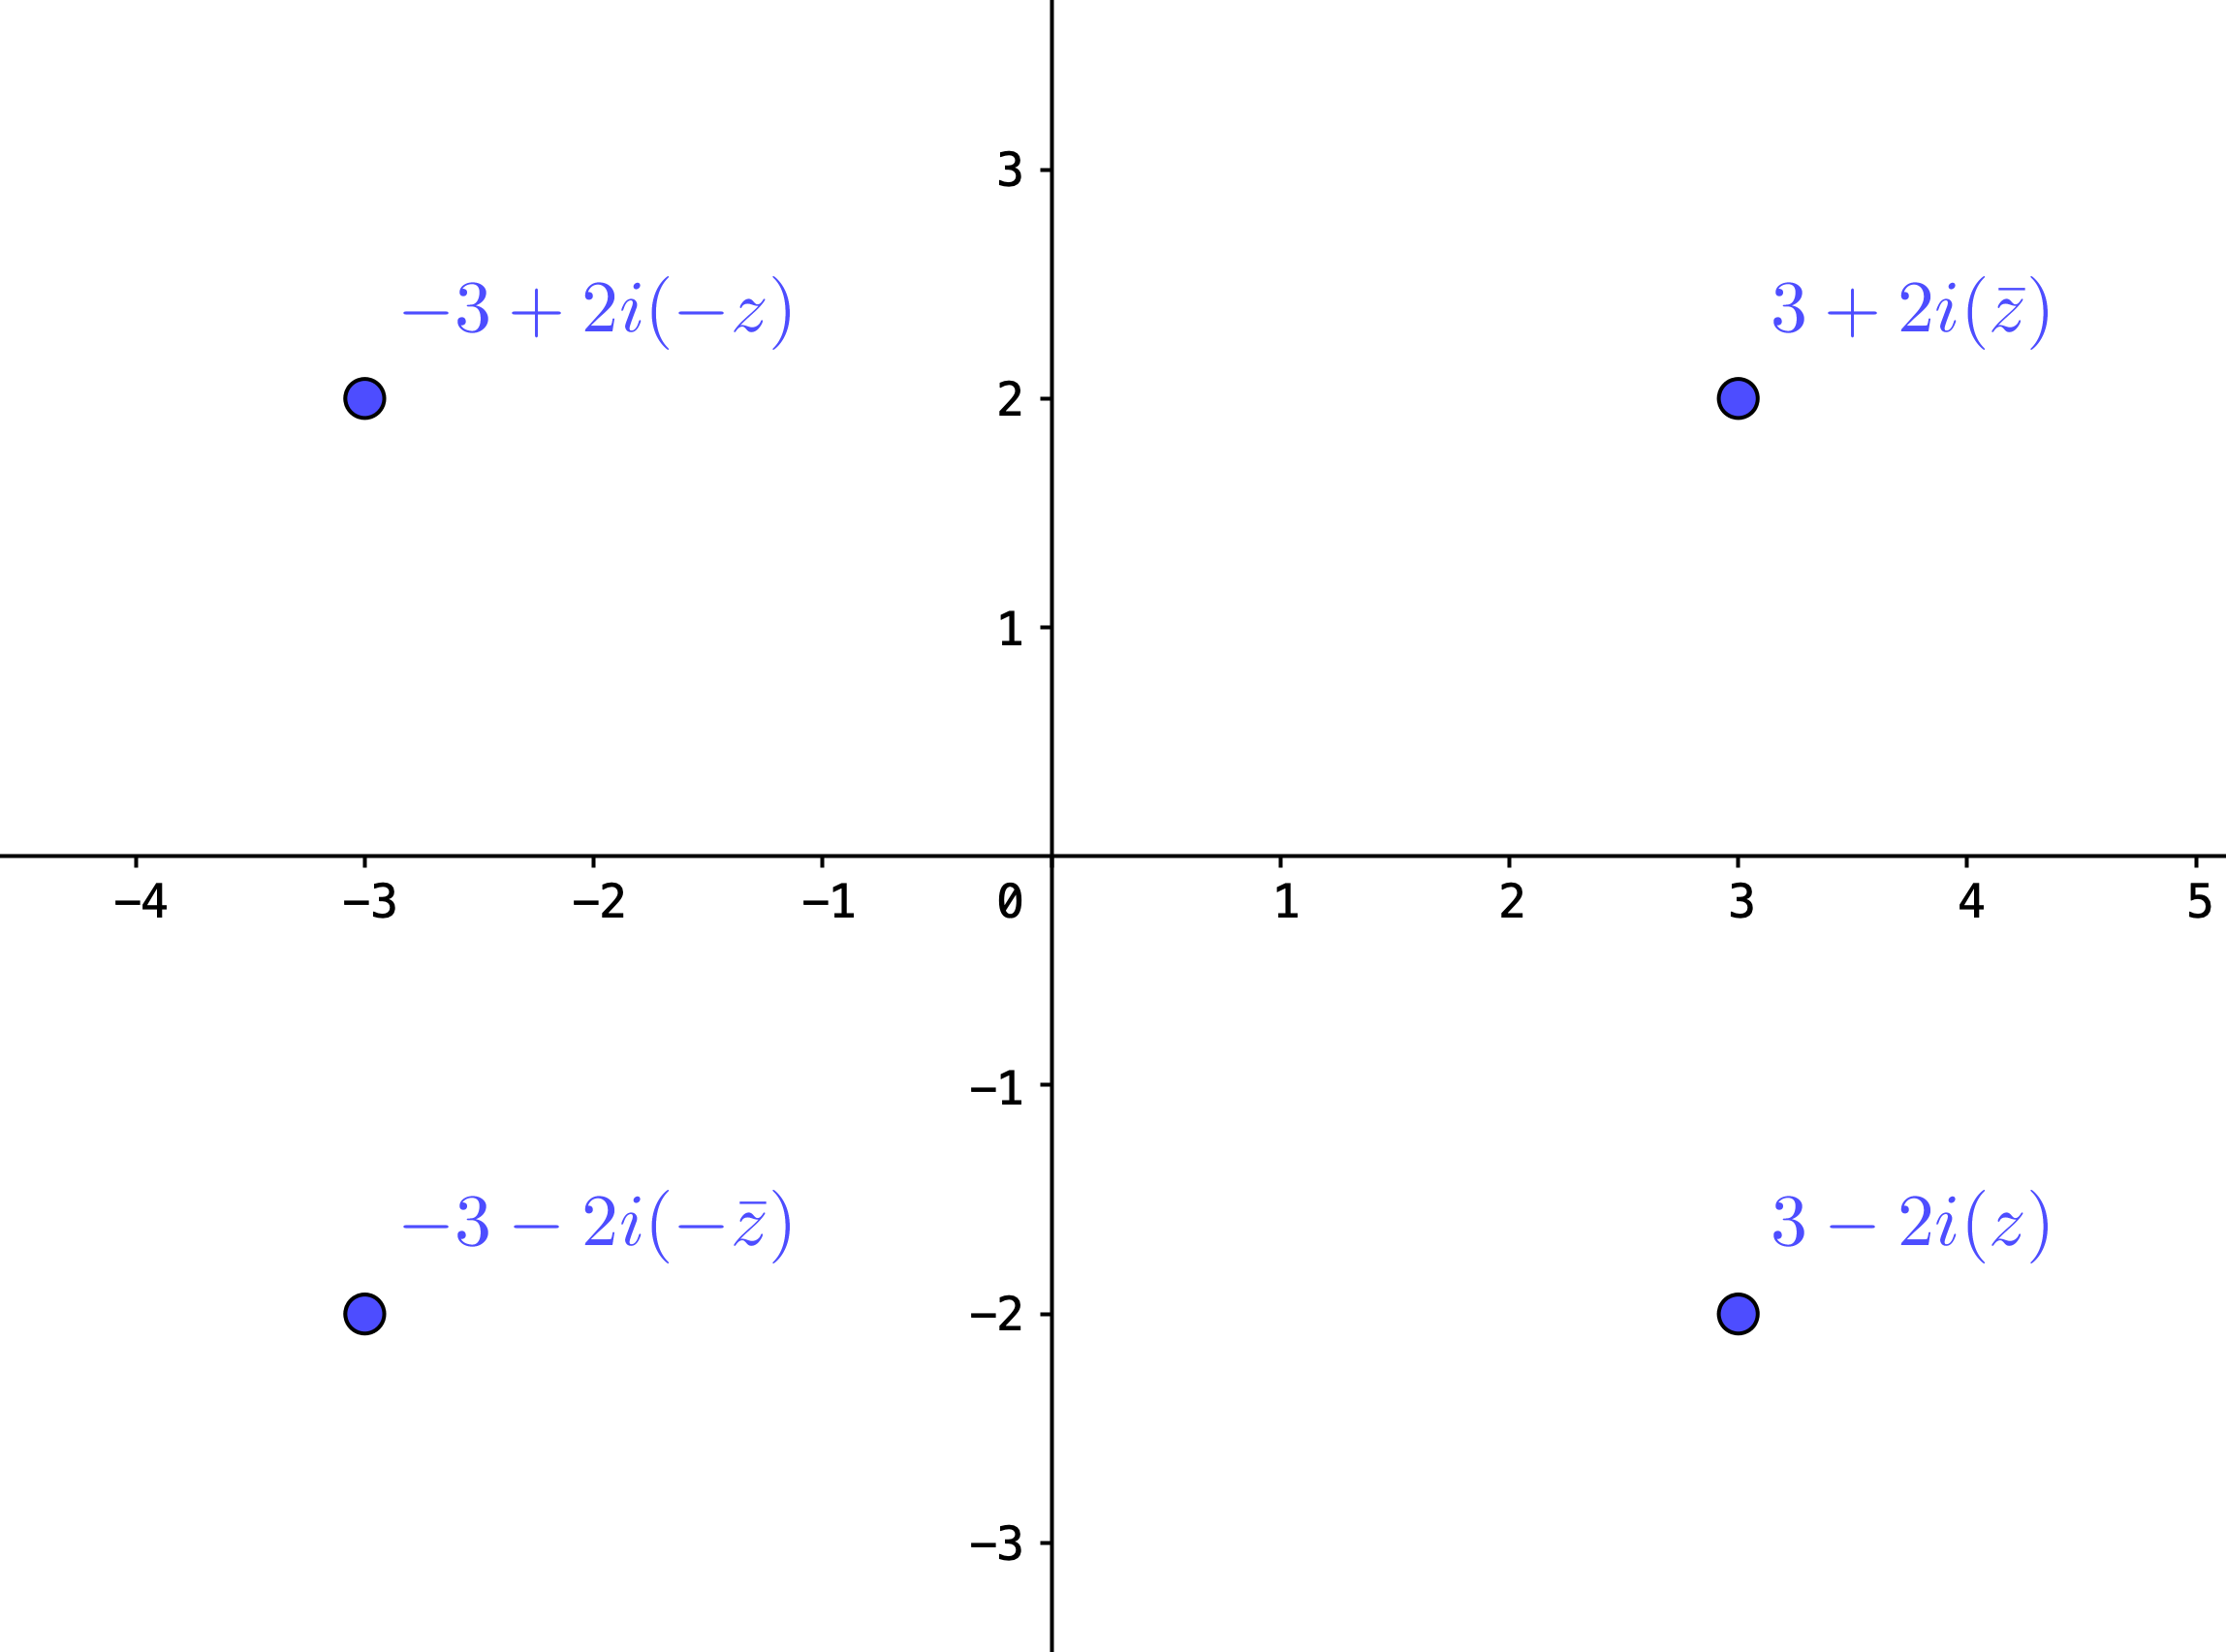
\includegraphics[width= .60 \textwidth]{plot1.png}
        \end{center}
    \end{figure}
    \begin{figure}[H]
        \begin{center}
        \caption{Plotting $z = 2 + 3i$}
        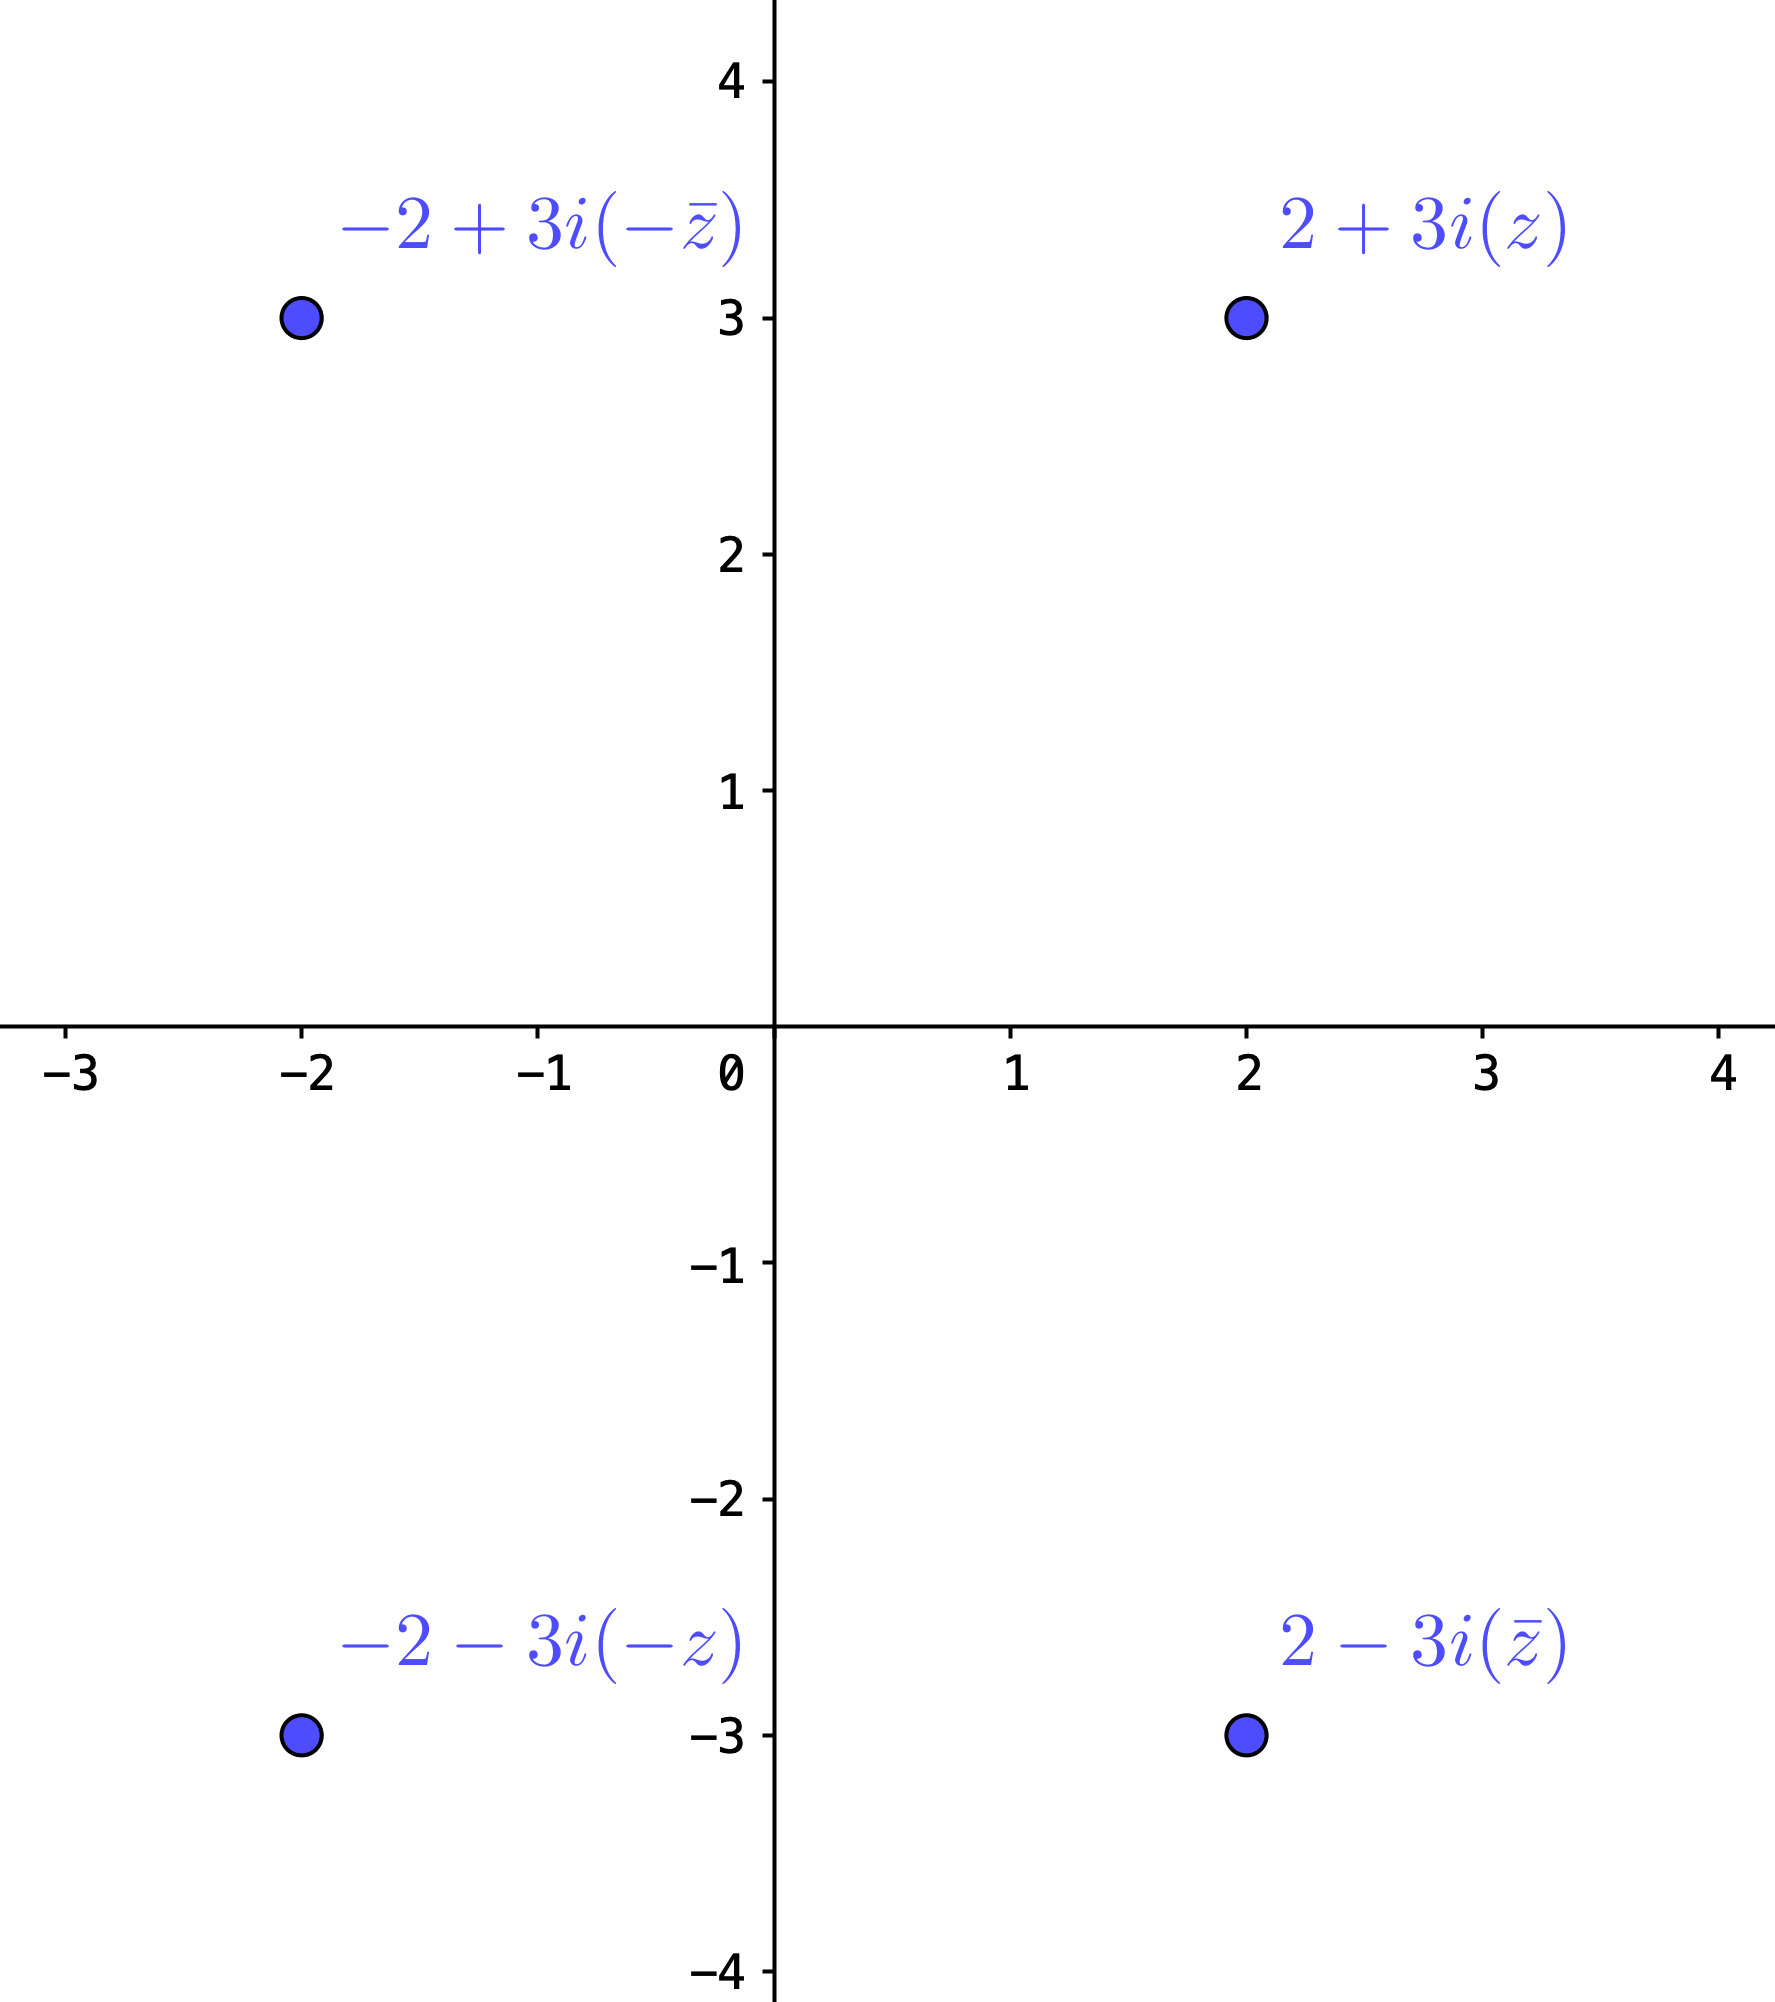
\includegraphics[width= .60 \textwidth]{plot2.png}
        \end{center}
    \end{figure}
    \begin{figure}[H]
        \begin{center}
        \caption{Plotting $z = -2i$}
        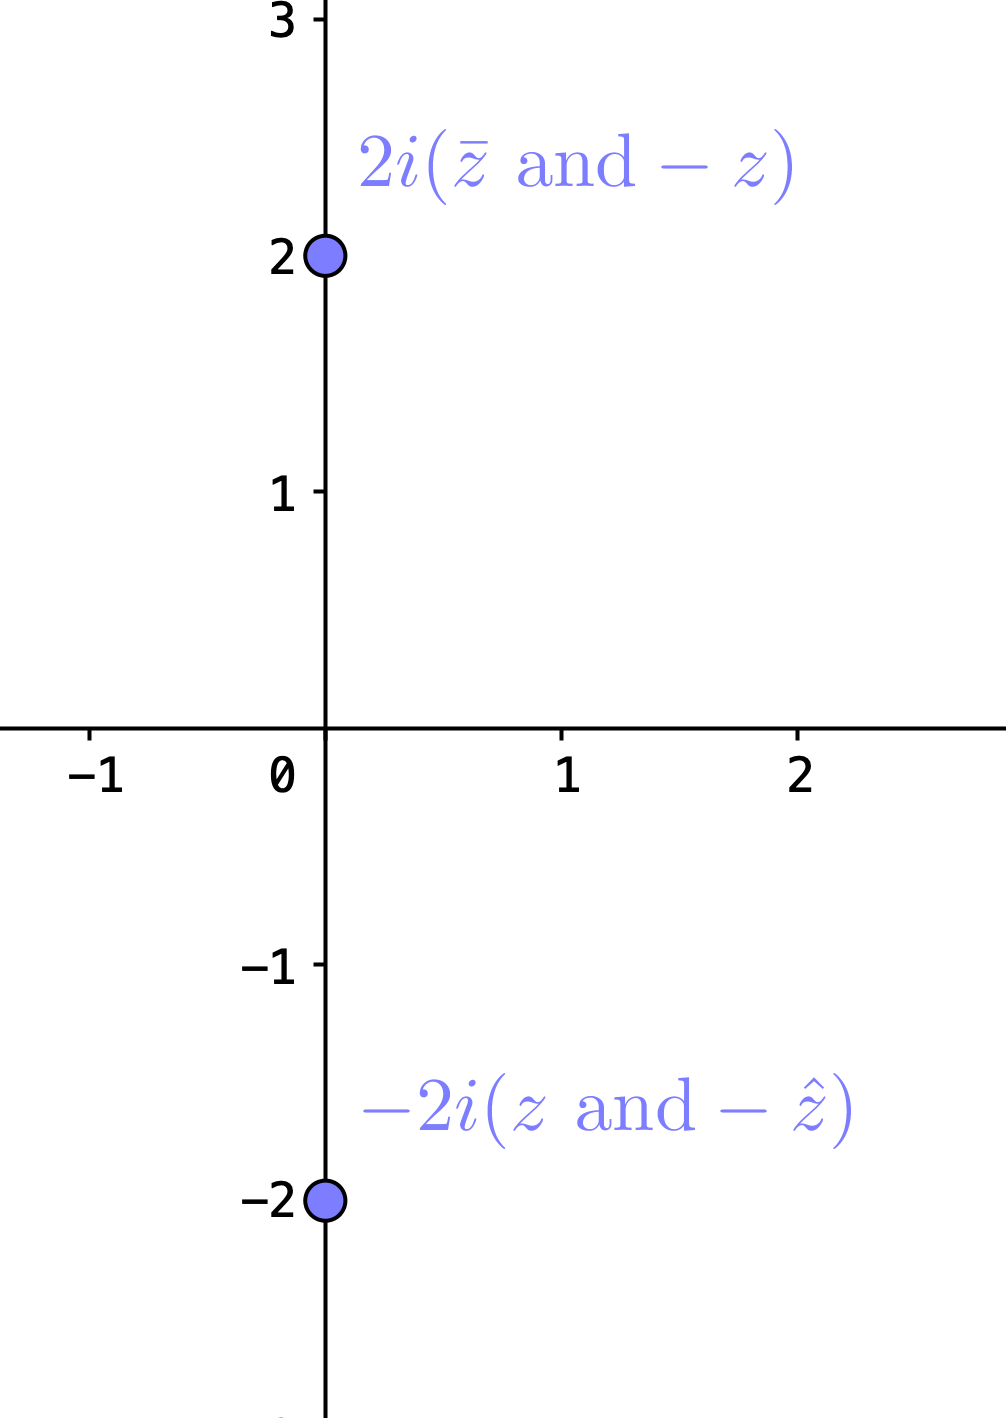
\includegraphics[width= .40 \textwidth]{plot3.png}
        \end{center}
    \end{figure}
\end{exercise}
\vspace{1in}



\begin{exercise}{7} Describe the set of points $z$ in the complex plane that satisfies each of the following, 
    \begin{enumerate}
        \item[a] $Im(z) = -2$\\
        \solution This plots a horizontal line across the complex plane parallel to the real numbers at a height of $-2$. 
        \vspace{.15in} 
        \item[c] $|2z - i| = 4$\\ 
        \solution Let $z = x + yi$ where $x, y \in \RR$. By substitution and through algebra we get, 
        \begin{align*}
            |2z - i| &= 4,\\
            |2(x + yi) - i| &= 4,\\
            |2x + (2y-1)i)| &= 4.
        \end{align*}
        Applying the definition of modulus, 
        \begin{align*}
            |2x + (2y-1)i)| &= 4,\\
            \sqrt{(2x)^2 + (2y-1)^2} &= 4,\\
            (2x)^2 + (2y-1)^2 &= 16.
        \end{align*}
       This final equation is a circle with radius 2 and center $(1, 0)$. 
        \vspace{.15in} 
        \item[h] $Re z\geq 4$\\
        \solution This plots the inequality where everything to the right side of a vertical line at $x = 4$ is shaded in. 
        \vspace{.15in} 
        \item[i]  $|z - i| < 2$\\
        \solution  Let $z = x + yi$ where $x, y \in \RR$. By substitution and through algebra we get, 
        \begin{align*}
            |z - i| &< 2,\\
            |x + (y-1)i| &< 2.
        \end{align*}
        Applying the definition of modulus, 
        \begin{align*}
            |x + (y-1)i| &< 2,\\
            \sqrt{x^2 + (y-1)^2} &< 2,\\
            x^2 + (y-1)^2 & < 4.
        \end{align*}
        This inequality describes all the points within the circle with radius 2 and center $(1, 0)$. 
    \end{enumerate}
\end{exercise}
\vspace{1in}


\begin{exercise}{8} Show both analytically and graphically, that $|z - 1| = |\bar{z} - 1|$. \\
    \solution Let $z = a + bi$, with $a, b \in \RR$. By definition $\bar{z} = a - bi$. By the definition of modulus, 
    \begin{equation*}
        |z - 1| = \sqrt{a^2 + b^2 - 1} = \sqrt{a^2 + (-b)^2 - 1} = |\bar{z} - 1|.
    \end{equation*}
    Graphically we know that the conjugate of a complex number $z$ simply reflects it about the real axis. Note that 
    $Re(z - 1) = Re(\bar{z} - 1)$, and $Im(z - 1) = -Im(\bar{z} - 1)$ so both numbers have the same distance from the origin, the 
    only difference being direction. 
\end{exercise}
\vspace{1in}



\begin{exercise}{12} Verify properties (3), (4), and (5) for $z_1$ and $z_2$. 
    First let $z_1 = a + bi$ and $z_2 = c + di$ for all $a, b, c, d \in \RR$. Demonstrating (3), consider 
    the division of complex numbers, 
    \begin{equation*}
        \overline{\left(\dfrac{z_1}{z_2}\right)} = \dfrac{ac + bd}{c^2 + d^2} - \dfrac{bc - ad}{c^2 + d^2}i = \dfrac{ac + bd}{c^2 + d^2} + \dfrac{(-b)c - a(-d)}{c^2 + d^2}i =   \dfrac{\bar{z_1}}{\bar{z_2}}
    \end{equation*}
    Demonstrating (4), let $z = a + bi$ and consider the following division, 
    \begin{equation*}
        \dfrac{z + \bar{z}}{2} = \dfrac{a + bi + a - bi}{2} = \dfrac{2a}{2} = a = Re(z). 
    \end{equation*}
    Similarly we can demonstrate (5) by considering the following, 
    \begin{equation*}
        \dfrac{z - \bar{z}}{2i} = \dfrac{a + bi - a - bi}{2i} = \dfrac{2bi}{2i} = b = Im(z). 
    \end{equation*}
\end{exercise}
\vspace{1in}





\begin{exercise}{13} Prove that if $(\bar{z})^2 = z^2$, then $z$ is either real or pure imaginary.\\
    \solution Let $z = a + bi$ for $a, b \in \RR$ and suppose that, $(\bar{z})^2 = z^2$. Expanding we get, 
    \begin{align*}
        (a - bi)^2 &= (a + bi)^2,
        (a - bi)(a - bi) &= (a + bi)(a + bi),\\
        a^2 - b^2 - 2abi &=  a^2 - b^2 + 2abi,\\
        0 = 4abi. 
    \end{align*}
    By the last product we know that either $Re(z) = a = 0$ which concludes that $z$ is pure imaginary or  $Im(z) = b = 0$ 
    which concludes that $z$ is real, or the case where $z = 0$. 
\end{exercise}
\vspace{1in}



\begin{exercise}{14} Prove that $|z_1z_2| = |z_1||z_2|$ (Hint: Use equations (7) and (2)).\\
    \solution Let $z_1$ and $z_2$ be complex numbers, and consider the square of the modulus of their product, $|z_1z_2|^2$.
    By equation (7) we know that the square fo the modulus of a complex number equals the number times its conjugate so we get the following, 
    \begin{equation*}
        |z_1z_2|^2 = z_1z_2 \overline{z_1z_2}
    \end{equation*}
    By equation (2) we can distribute the conjugate among the right hand side product to get, 
    \begin{equation*}
        |z_1z_2|^2 = z_1z_2 \overline{z_1}\overline{z_2}.
    \end{equation*}
    Since complex multiplication is commutative we can reorder the product and apply equation (7) to simplify, 
    \begin{align*}
        |z_1z_2|^2 &= z_1z_2 \overline{z_1}\overline{z_2},\\
        |z_1z_2|^2 &= z_1\overline{z_1} z_2\overline{z_2},\\
        |z_1z_2|^2 &= |z_1|^2|z_2|^2,\\
        |z_1z_2| &= |z_1||z_2|.\\
    \end{align*}
\end{exercise}

\begin{exercise}{15} Prove that $(\bar{z})^k = \overline{(z^k)}$ for every integer $k$ (provided $z \neq 0$ when $k$ is negative.)\\
    \solution Suppose some complex number $z$ let $k \in k \in \mathbb{Z}^+$. Note that the case where $k = 0$ is trivial. Consider the case where $k = 1$ and note that, 
    \begin{align*}
        (\bar{z})^1 &= \overline{(z^1)},\\
        \bar{z} &= \bar{z}. 
    \end{align*}
    Suppose  $(\bar{z})^k = \overline{(z^k)}$ for some $k$ and we will proceed by induction on $k$. Consider the following. 
    \begin{equation*}
        (\bar{z})^{k+1} = (\bar{z})^k(\bar{z}).
    \end{equation*}
    By the induction hypothesis we know that,
    \begin{equation*}
        (\bar{z})^{k+1} = \overline{(z^k)}(\bar{z}) =  \overline{(z^k)(z)} = \overline{(z^{k+1})}.
    \end{equation*}
    For the case where $k \in \mathbb{Z}^-$, consider the previous result and with some algebra we get,
    \begin{align*}
        (\bar{z})^k &= \overline{(z^k)},\\
        {(\bar{z})^{k}}^{-1} &= {\overline{(z^{k})}}^{-1},\\
        (\bar{z})^{(-1)k} &= \overline{(z^{(-1)k})}.
    \end{align*}
\end{exercise}



\end{document}


















